\documentclass[10pt]{article}

\usepackage[T1]{fontenc}
\usepackage[left=2cm, right=2cm, top=2cm, bottom=2cm, paperheight=31cm]{geometry}
\usepackage[skins]{tcolorbox}
\usepackage{hyperref, fancyhdr, lastpage, tocloft, ragged2e, multicol, changepage}
\usepackage{amsmath, amssymb, amsthm, stmaryrd}
\usepackage{tkz-tab}
\usepackage{systeme}

\def\pagetitle{Suites, La Pratique}
\setlength{\headheight}{13pt}

\title{\bf{\pagetitle}\\\large{Corrigé}}
\date{Novembre 2023}
\author{DARVOUX Théo}

\DeclareMathOperator{\ch}{ch}

\hypersetup{
    colorlinks=true,
    citecolor=black,
    linktoc=all,
    linkcolor=blue
}

\pagestyle{fancy}
\cfoot{\thepage\ sur \pageref*{LastPage}}


\begin{document}
\renewcommand*\contentsname{Exercices.}
\renewcommand*{\cftsecleader}{\cftdotfill{\cftdotsep}}
\maketitle

\hrule
\tableofcontents
\vspace{0.5cm}
\hrule


\thispagestyle{fancy}
\fancyhead[L]{MP2I Paul Valéry}
\fancyhead[C]{\pagetitle}
\fancyhead[R]{2023-2024}
\allowdisplaybreaks

\pagebreak


\section*{Exercice 13.1 [$\blacklozenge\lozenge\lozenge$]}
\begin{tcolorbox}[enhanced, width=7.6in, center, size=fbox, fontupper=\large, drop shadow southwest]
    Une suite croissante est une fonction croissante sur $\mathbb{N}$.\\
    Démontrer que le titre de l'exercice dit vrai, c'est-à-dire, pour une suite réelle $(u_n)_{n\in\mathbb{N}}$ l'équivalence entre\\
    1. $\forall{n\in\mathbb{N}} ~ u_{n+1} \geq u_n$.\\
    2. $\forall{(n,p)\in\mathbb{N}^2} ~ n \leq p \Longrightarrow u_n \leq u_p$.\\[0.1cm]
    Supposons 2, montrons 1.\\
    Soit $n\in\mathbb{N}$\\
    On a $n\leq n+1$. D'après 2, $u_n \leq u_{n+1}$. ez\\[0.1cm]
    Supposons 1, montrons 2.\\
    Soit $(n, p)\in\mathbb{N}^2$ tels que $n \leq p$. On sait que $u_{n+1} \geq u_n$, $u_{n+2} \geq u_{n+1}$, $u_{n+3} \geq u_{n+2}$, etc...\\
    Par récurrence triviale et par transitivité, pour tout entier $q\geq n$, $u_q \geq u_n$.\\
    En particulier, $u_p \geq u_n$\\
    \qed
\end{tcolorbox}
\addcontentsline{toc}{section}{Avant de parler de convergence.}
\addcontentsline{toc}{section}{\protect\numberline{}Exercice 13.1}

\section*{Exercice 13.2 [$\blacklozenge\blacklozenge\lozenge$]}
\begin{tcolorbox}[enhanced, width=7.6in, center, size=fbox, fontupper=\large, drop shadow southwest]
    Soit $a$ un réel supérieur à 1 et $(u_n)_{n\geq0}$ la suite définie par $\forall n \in \mathbb{N} ~ u_n = \frac{a^n}{n!}$.\\
    Démontrer que l'ensemble des termes de la suite possède un maximum, qu'on exprimera en fonction de $a$.\\
    $(u_n)$ est strictement positive sur $\mathbb{N}$.\\
    Soit $n \in \mathbb{N}$.\\
    On peut donc écrire : $\frac{u_{n+1}}{u_n}=\frac{a}{n+1}$.\\
    Ainsi, $(u_n)$ est croissante ($a\geq n+1$) puis décroissante ($a\leq n+1$), ce qui implique qu'un maximum existe.\\
    Ce maximum est atteint lorsque $a=n+1$ c'est à dire quand $n=\lfloor a \rfloor$.\\
    Ainsi, le maximum de la suite $u$ est : $\frac{a^{\lfloor a \rfloor}}{\lfloor a \rfloor!}$\\
    \qed
\end{tcolorbox}

\addcontentsline{toc}{section}{\protect\numberline{}Exercice 13.2}

\section*{Exercice 13.3 [$\blacklozenge\lozenge\lozenge$]}
\begin{tcolorbox}[enhanced, width=7.6in, center, size=fbox, fontupper=\large, drop shadow southwest]
    Pour $n\in\mathbb{N}$, on pose
    \begin{equation*}
        u_n = \sum_{k=n+1}^{2n}\frac{k\sin k}{k^2+1}.
    \end{equation*}
    Prouver que la suite $(u_n)$ est bornée.\\
    Soit $n\in\mathbb{N}$, on a : $-1 \leq \sin n \leq 1$. Donc :
    \begin{align*}
        \left|\sum_{k=n+1}^{2n}\frac{k\sin k}{k^2+1}\right| &\leq \sum_{k=n+1}^{2n}\frac{k}{k^2+1}\\
        &\leq \sum_{k=n+1}^{2n}\frac{n+1}{(n+1)^2+1}\\
        &\leq \frac{n^2 + n}{n^2 + 2n + 2}\\
        &\leq 1
    \end{align*}
    Majorer en valeur absolue c'est borner\\
    \qed
\end{tcolorbox}

\addcontentsline{toc}{section}{\protect\numberline{}Exercice 13.3}

\section*{Exercice 13.4 [$\blacklozenge\lozenge\lozenge$]}
\begin{tcolorbox}[enhanced, width=7.6in, center, size=fbox, fontupper=\large, drop shadow southwest]
    Soit $\alpha\in]0,1[$ et $(u_n)$ la suite définie par $\begin{cases}
        u_0 = \alpha(1-\alpha)\\
        \forall n \geq 0 ~ u_{n+1}=(1-\alpha)u_n + \alpha(1-\alpha)
    \end{cases}$\\
    1. Exprimer le terme général de la suite en fonction de $\alpha$ et $n$.\\
    2. Donner $\lim u_n$.\\[0.1cm]
    1. Soit $n\in\mathbb{N}$.\\
    On pose l'équation au point fixe : $x = (1-\alpha)x + \alpha(1-\alpha)$.\\
    Sa solution est : $x=1-\alpha$.\\
    On a : $u_{n+1} - (1 - \alpha) = (1-\alpha)u_n + \alpha(1-\alpha) - (1 - \alpha)$.\\
    Ainsi, $u_{n+1} + \alpha - 1 = (1-\alpha)(u_n + \alpha - 1)$.\\
    On pose $v_n := u_n + \alpha - 1$. Par définition, $v$ est géométrique, de raison $1-\alpha$.\\
    Son terme général est : $v_n=v_0(1-\alpha)^n$.\\
    Or $v_0=u_0 + \alpha - 1 = \alpha(1-\alpha) + \alpha - 1 = (\alpha-1)(1-\alpha)$.\\
    On en déduit que $v_n = (\alpha-1)(1-\alpha)^{n+1}$.\\
    Finalement, $u_n=(\alpha-1)(1-\alpha)^{n+1}-\alpha+1$.\\
    \qed
\end{tcolorbox}

\addcontentsline{toc}{section}{\protect\numberline{}Exercice 13.4}

\section*{Exercice 13.5 [$\blacklozenge\lozenge\lozenge$]}
\begin{tcolorbox}[enhanced, width=7.6in, center, size=fbox, fontupper=\large, drop shadow southwest]
    Soit $\theta\in\mathbb{R}$.\\
    1. Donner la forme du terme général d'une suite $(u_n)_{n\in\mathbb{N}}$ de $\mathbb{R}^\mathbb{N}$ telle que
    \begin{equation*}
        \forall n \in \mathbb{N} ~ u_{n+2} - 2\cos(\theta)u_{n+1} + u_n = 0.
    \end{equation*}
    2. Supposons dans cette question que $\theta \notin \pi\mathbb{Z}$. Donner sous forme factorisée le terme général de l'unique suite $(u_n)$ satisfaisant la relation ci-dessus et telle que $u_0=u_1=1$.\\[0.1cm]
    Polynome caractéristique : $r^2 - 2\cos(\theta)r + 1$. $\Delta = -4\sin^2(\theta)$. $r_1 = \cos(\theta) + i\sin(\theta)$ et $r_2 = \cos(\theta) - i\sin(\theta)$.\\
    Lorsque $\theta\in\pi\mathbb{Z}$: $\exists!(\lambda,\mu)\in\mathbb{R}^2 ~ \forall n\in\mathbb{N}, ~ u_n = \lambda n \cos^n(\theta) + \mu \cos^n(\theta)$.\\
    Lorsque $\theta\notin\pi\mathbb{Z}$: $\exists!(\lambda,\mu)\in\mathbb{R}^2 ~ \forall n\in\mathbb{N}, ~ u_n = \lambda \cos(n\theta) + \mu\sin(n\theta)$.\\
    2. Soient $\lambda,\mu\in\mathbb{R}$ tels que $\forall n\in\mathbb{N}, ~ u_n = \lambda\cos(n\theta)+\mu\sin(n\theta)$.\\
    On a $u_0 = \lambda = 1$ et $u_1 = \cos(\theta) + \mu\sin(\theta) = 1$ donc $\mu = \frac{1-\cos(\theta)}{\sin(\theta)}$.\\
    Ainsi, $\forall n\in\mathbb{N}n, ~ u_n = \cos(n\theta) + \frac{1-\cos(\theta)}{\sin(\theta)}\sin(n\theta)$\\
    \emph{Comment tu factorises ça wtf}\qed
\end{tcolorbox}

\addcontentsline{toc}{section}{\protect\numberline{}Exercice 13.5}

\section*{Exercice 13.6 [$\blacklozenge\blacklozenge\lozenge$]}
\begin{tcolorbox}[enhanced, width=7.6in, center, size=fbox, fontupper=\large, drop shadow southwest]
    Soit $(u_n)$, définie par récurrence par $\begin{cases}u_0=1\\\forall n \geq 0, ~ u_{n+1} = 3u_n + 2^n\end{cases}$.\\
    1. Prouver qu'il existe une suite $(a_n)$ géométrique de raison 2 qui satisfait la relation de récurrence.\\
    2. Donner le terme général de $(u_n)$.\\[0.1cm]
    1. Soit $n\in\mathbb{N}$ et soit $(a_n)$ une suite géométrique de raison 2. On a :
    \begin{equation*}
        \forall n\in\mathbb{N}, ~ a_n = a_02^{n}
    \end{equation*}
    On cherche $(a_n)$ telle que $a_{n+1} = 3a_n + 2^n = 3a_02^n+2^n = 2^n(3a_0+1)$.\\
    Posons $a_0 = -1$. On a $a_{n+1} = 2^n(-2) = -2^{n+1} = a_02^{n+1}$.\\
    Ainsi, la suite géométrique $(a_n)$ de raison 2 et de premier terme $-1$ satisfait la relation de récurrence.\\
    2. On a $u_{n+1} - 2a_n = 3u_n + 2^n - 2a_n \iff u_{n+1} - a_{n+1} = 3(u_n - a_n)$.\\
    On pose $v_n := u_n - a_n$. Alors $v_0 = u_0 - a_0 = 2$ et $v_n = 2\cdot3^n$.\\
    On en déduit que $u_n = v_n + a_n = 2\cdot3^n - 2^n = 2(3^n - 2^{n-1})$\\
    On a $u_{n+1} = 2(3^{n+1} - \cdot2^{n})$ \qed
\end{tcolorbox}

\addcontentsline{toc}{section}{\protect\numberline{}Exercice 13.6}

\section*{Exercice 13.7 [$\blacklozenge\blacklozenge\lozenge$]}
\begin{tcolorbox}[enhanced, width=7.6in, center, size=fbox, fontupper=\large, drop shadow southwest]
    Étudier la suite $(u_n)$, définie par récurrence par $\begin{cases}
        u_0 > 0; u_1 > 0\\
        \forall n \geq 0 ~ u_{n+2} = \sqrt{u_{n+1}u_n}
    \end{cases}$.\\
    Soit $n\in\mathbb{N}$.\\
    On a :
    \begin{align*}
        u_{n+2} = \sqrt{u_{n+1}u_n} &\iff \ln(u_{n+2}) = \ln(\sqrt{u_{n+1}u_n})\\
        &\iff \ln(u_{n+2}) = \frac{1}{2}(\ln(u_{n+1}) + \ln(u_n))
    \end{align*}
    On pose $v_n := \ln(u_n)$.\\
    On obtient : $v_{n+2} = \frac{1}{2}v_{n+1} + \frac{1}{2}v_n$.\\
    C'est une suite récurrente linéaire d'ordre 2 !\\
    Polynome caractéristique : $r^2 - \frac{1}{2}r - \frac{1}{2}$. $\Delta = \frac{9}{4}$. $r_1 = 1$ et $r_2 = -\frac{1}{2}$.\\
    Ainsi, $v_n = \lambda + \frac{\mu(-1)^n}{2^n} ~ | ~ (\lambda, \mu)\in\mathbb{R}^2$.\\
    Soient $(\lambda,\mu)\in\mathbb{R}^2$ et $v_n$ une telle suite.\\
    Alors $v_0 = \lambda + \mu$ et $v_1 = \lambda - \frac{\mu}{2}$.\\
    On a $v_0 + 2v_1 = 3\lambda = \ln(u_0u_1^2)$. Donc $\lambda = \ln(\sqrt[3]{u_0u_1^2})$.\\
    On a $u_n = e^\lambda \cdot e^{\frac{\mu(-1)^n}{2^n}} \to e^{\lambda}$. Ainsi, $u_n \to \sqrt[3]{u_0u_1^2}$.\\
    \qed
\end{tcolorbox}

\addcontentsline{toc}{section}{\protect\numberline{}Exercice 13.7}

\section*{Exercice 13.8 [$\blacklozenge\lozenge\lozenge$]}
\begin{tcolorbox}[enhanced, width=7.6in, center, size=fbox, fontupper=\large, drop shadow southwest]
    Soit $a>1$. Pour $n\geq1$, on définit $u_n=(\lfloor a^n \rfloor)^{1/n}$.\\
    Montrer que $(u_n)$ est convergente et donner sa limite.\\
    On a :
    \begin{align*}
        a^n - 1 < \lfloor a^n \rfloor \leq a^n &\iff (a^n - 1)^{\frac{1}{n}} < \lfloor a^n \rfloor ^ \frac{1}{n} \leq a
    \end{align*}
    On peut appliquer la fonction $x\mapsto \frac{1}{n}$ : elle est croissante sur $\mathbb{R}_+$ et $a>1$.\\
    D'une part, $(a^n - 1)^{\frac{1}{n}} = (a^n(1 - \frac{1}{a^n}))^{\frac{1}{n}} = a(1-\frac{1}{a^n})^\frac{1}{n} \to a$.\\
    D'autre part, $a \to a$ (\emph{big brain})\\
    Ainsi, d'après le théorème des gendarmes : $\lfloor a^n \rfloor ^ \frac{1}{n} \to a$.\\
    \qed
\end{tcolorbox}


\addcontentsline{toc}{section}{Encadrement.}
\addcontentsline{toc}{section}{\protect\numberline{}Exercice 13.8}
\section*{Exercice 13.9 [$\blacklozenge\blacklozenge\lozenge$]}
\begin{tcolorbox}[enhanced, width=7.6in, center, size=fbox, drop shadow southwest]
    Pour tout $n\in\mathbb{N}^*$, on note $u_n=\prod\limits_{k=1}^{n}\left( 1 + \frac{k}{n^2} \right)$.\\
    1. Montrer que pour tout $x\geq0$, $x-\frac{x^2}{2} \leq \ln(1+x) \leq x$.\\
    2. Montrer que $u$ converge et déterminer sa limite.\\[0.1cm]
    Soit $x\in\mathbb{R}_+$.\\
    1. On pose $f:x\mapsto\ln(1+x) - x$. $f$ est dérivable comme somme et $f':x\mapsto-\frac{x}{1+x}$. $f$ décroissante sur $\mathbb{R}_+$.\\
    Or $f(0)=0$ donc $f(x)\leq0$. Ainsi, $\ln(1+x) \leq x$.\\[0.1cm]
    On pose $g:x\mapsto x-\frac{x^2}{2} - \ln(1+x)$. $g$ est dérivable comme somme, $g':x\mapsto -\frac{x^2}{1+x}$. $g$ décroissante sur $\mathbb{R}_+$.\\
    Or $g(0)=0$ donc $g(x)\leq0$. Ainsi, $x - \frac{x^2}{2} \leq \ln(1+x)$.\\[0.1cm]
    2. Posons $v_n := \ln(u_n)$. Alors $v_n = \sum\limits_{k=1}^n\ln\left( 1+\frac{k}{n^2} \right)$.\\
    Alors $\sum\limits_{k=1}^n(\frac{k}{n^2}-\frac{k^2}{2n^4}) \leq v_n \leq \sum\limits_{k=1}^n\frac{k}{n^2}$ : $\frac{n+1}{2n} - \frac{(n+1)(2n+1)}{12n^3}\leq v_n \leq \frac{n+1}{2n}$.\\
    Par théorème des gendarmes, $v_n \to \frac{1}{2}$. Ainsi, $u_n \to \sqrt{e}$.\\
    \qed
\end{tcolorbox}

\addcontentsline{toc}{section}{\protect\numberline{}Exercice 13.9}

\section*{Exercice 13.10 [$\blacklozenge\blacklozenge\blacklozenge$]}
\begin{tcolorbox}[enhanced, width=7.6in, center, size=fbox, fontupper=\large, drop shadow southwest]
    Étudier la convergence de la suite de terme général $\frac{1! + 2! + ... + n!}{n!}$.\\
    Soit $(u_n)$ une suite de terme général : $\frac{1}{n!}\sum_{k=1}^nk!$.\\
    Soit $n\in\mathbb{N}$.\\
    On sait d'avance que $u_n \geq 1$, puisque $\sum_{k=1}^nk! \geq n!$.\\
    De plus,
    \begin{align*}
        \frac{1}{n!}\sum_{k=1}^nk! &= \frac{n!}{n!} + \frac{(n-1)!}{n!} + \frac{1}{n!}\sum_{k=1}^{n-2}k!\\
        &\leq 1 + \frac{1}{n} + \frac{(n-2)(n-2)!}{n!}\\
        &= 1 + \frac{1}{n} + \frac{n-2}{n(n-1)}\\
        &\longrightarrow 1 
    \end{align*}
    D'après le théorème des gendarmes (AQAB), $u_n \to 1$.\\
    \qed 
\end{tcolorbox}

\addcontentsline{toc}{section}{\protect\numberline{}Exercice 13.10}

\section*{Exercice 13.11 [$\blacklozenge\lozenge\lozenge$]}
\begin{tcolorbox}[enhanced, width=7.6in, center, size=fbox, fontupper=\large, drop shadow southwest]
    Pour $n\in\mathbb{N}$, on pose $I_n = \int_0^{\frac{\pi}{4}}(\arctan(x))^ndx$. Justifier que $(I_n)$ est convergente.\\
    Soit $n\in\mathbb{N}$.\\
    Pour $x\in[0, \frac{\pi}{4}]$, on a $\arctan(x)^n \in [0,1]$ donc $\arctan^{n+1}(x) \leq \arctan^n(x)$.\\
    Alors :
    \begin{align*}
        I_{n+1} - I_n = \int_0^{\frac{\pi}{4}}\left( \arctan^{n+1}(x) - \arctan^n(x) \right)dx \leq 0.
    \end{align*}
    Ainsi, $I_n$ est décroissante et minorée par 0 : $I_n$ est convergente d'apres le TLM.\\
    \qed
\end{tcolorbox}
\addcontentsline{toc}{section}{Monotonie.}
\addcontentsline{toc}{section}{\protect\numberline{}Exercice 13.11}

\section*{Exercice 13.12 [$\blacklozenge\lozenge\lozenge$]}
\begin{tcolorbox}[enhanced, width=7.6in, center, size=fbox, fontupper=\large, drop shadow southwest]
    Soit $\alpha$ un réel de $]0,1[$. Pour tout $n\in\mathbb{N}^*$, on pose $u_n=\prod_{k=1}^n(1+\alpha^k)$.\\
    1. Justifier brièvement que $\forall x \in \mathbb{R} ~ 1 + x \leq e^x$.\\
    2. Démontrer que $(u_n)$ est une suite convergente, et que $\lim u_n \leq \exp(\frac{\alpha}{1-\alpha})$.\\[0.1cm]
    1. Soit $x\in\mathbb{R}$, par convexité de l'exponentielle, elle est supérieure à toutes ses tangentes, en particulier $x+1$.\\
    2. Puisque $\forall x\in\mathbb{R}, ~ 1 + x \leq e^x$, on a $\forall k\in\mathbb{N}, ~ 1 + \alpha^k \leq e^{\alpha^k}$.\\
    Ainsi :
    \begin{align*}
        \prod_{k=1}^n(1+\alpha^k) \leq \prod_{k=1}^ne^{\alpha^k}=\exp(\sum_{k=1}^n{\alpha^k})=\exp(\frac{\alpha-\alpha^{n+1}}{1-\alpha})\leq\exp\left( \frac{\alpha}{1-\alpha} \right)
    \end{align*}
    On a $u_n>0$ donc on peut écrire :
    \begin{align*}
        \frac{u_{n+1}}{u_n} = 1+\alpha^{n+1} > 1
    \end{align*}
    Donc $(u_n)$ est croissante et majorée, ainsi elle converge vers un réel $l \leq \exp(\frac{\alpha}{1-\alpha})$\\
    \qed
\end{tcolorbox}
\addcontentsline{toc}{section}{\protect\numberline{}Exercice 13.12}

\section*{Exercice 13.13 [$\blacklozenge\lozenge\lozenge$]}
\begin{tcolorbox}[enhanced, width=7.6in, center, size=fbox, fontupper=\large, drop shadow southwest]
    Soient $(u_n)$ et $(v_n)$ deux suites définies par
    \begin{equation*}
        \forall n \in \mathbb{N}^* \quad u_n = \sum_{k=n+1}^{2n}\frac{1}{k} ~ et ~ v_n = u_n + \frac{1}{n}.
    \end{equation*}
    Démontrer que $(u_n)$ et $(v_n)$ convergent vers une même limite.\\
    Soit $n\in\mathbb{N}$.\\
    On a :
    \begin{align*}
        &u_{n+1} - u_n = \sum_{k=n+2}^{2n+2}\frac{1}{k} - \sum_{k=n+1}^{2n}\frac{1}{k}=\frac{1}{2n+2} + \frac{1}{2n+1} - \frac{1}{n+1} = \frac{1}{4n^2 + 6n + 2} > 0\\
        &v_{n+1} - v_n = u_{n+1} + \frac{1}{n+1} - u_{n} - \frac{1}{n} = \frac{1}{2n+2} + \frac{1}{2n+1} - \frac{1}{n} = -\frac{3n+2}{2n(n+1)(2n+1)}<0
    \end{align*}
    Alors $(u_n)$ et $(v_n)$ sont monotones de monotonies contraires.\\
    On a :
    \begin{align*}
        u_n - v_n = -\frac{1}{n} \longrightarrow 0
    \end{align*}
    Ainsi, $(u_n)$ et $(v_n)$ sont adjacentes : elles convergent vers la même limite.\\
    \qed
\end{tcolorbox}
\addcontentsline{toc}{section}{\protect\numberline{}Exercice 13.13}

\section*{Exercice 13.14 [$\blacklozenge\blacklozenge\lozenge$]}
\begin{tcolorbox}[enhanced, width=7.6in, center, size=fbox, fontupper=\large, drop shadow southwest]
    Soient $(u_n)$ et $(v_n)$ deux suites définies par $u_0 > v_0 > 0$ et
    \begin{equation*}
        u_{n+1} = \frac{u_n + v_n}{2}; ~ v_{n+1} = \frac{2u_nv_n}{u_n + v_n}.
    \end{equation*}
    Montrer que ces deux suites convergent vers une limite commune. En examinant la suite $(u_nv_n)$, exprimer cette limite en fonction de $u_0$ et $v_0$.\\
    Soit $n\in\mathbb{N}$. On a $u_{n+1} - u_n = \frac{v_n - u_n}{2}$. Montrons $\mathcal{P}_n$ : <<$v_n-u_n \leq 0$>>.\\
    $\mathcal{P}_0$ est évident. On suppose $\mathcal{P}_n$ pour un $n$ fixé. Montrons $\mathcal{P}_{n+1}$.\\
    On a $v_{n+1} - u_{n+1} = \frac{2u_nv_n}{u_n+v_n} - \frac{u_n+v_n}{2} = \frac{2u_nv_n - u_n^2 - v_n^2}{2(u_n + v_n)}=-\frac{(u_n - v_n)^2}{2(u_n + v_n)}\leq0$.\\
    $\mathcal{P}_{n+1}$ est vrai. Par récurrence, $\mathcal{P}_n$ est vrai pour tout $n\in\mathbb{N}$.\\
    On a $v_{n+1} - v_n = \frac{2u_nv_n}{u_n+v_n} - \frac{v_n(u_n + v_n)}{u_n + v_n}=\frac{v_n(u_n - v_n)}{u_n + v_n}\geq0$.\\
    Ainsi, $u$ est décroissante, $v$ est croissante.\\
    $u$ est minorée par $0$ : elle converge vers une limite $l\in\mathbb{R}$.\\
    Puisque $u_{n+1}v_{n+1} = \frac{u_n+v_n}{2}\cdot\frac{2u_nv_n}{u_n+v_n}=u_nv_n$, $(u_nv_n)$ est constante et $u_nv_n = u_0v_0$.\\
    On obtient que $v_n$ converge aussi vers une limite $m\in\mathbb{R}$.\\
    On a : $u_{n+1} = \frac{u_n + v_n}{2} \longrightarrow \frac{l + m}{2}$.\\
    Ainsi, $l = \frac{l + m}{2}$ donc $l = m$. Les deux suites convergent vers la même limite.\\
    Puisque $u_nv_n = u_0v_0$, $lm = u_0v_0$ donc $l = m = \sqrt{u_0v_0}$\\
    \qed
\end{tcolorbox}
\addcontentsline{toc}{section}{\protect\numberline{}Exercice 13.14}

\section*{Exercice 13.15 [$\blacklozenge\blacklozenge\lozenge$]}
\begin{tcolorbox}[enhanced, width=7.6in, center, size=fbox, fontupper=\large, drop shadow southwest]
    Pour $n\in\mathbb{N}^*$
    \begin{equation*}
        u_n = \sum_{k=1}^{n}\frac{1}{k} \quad \text{et} \quad v_n = \sum_{k=1}^{n}\frac{1}{k^2}
    \end{equation*}
    1. Pour chacune des deux suites $u$ et $v$, faire un pronostic : convergente ou divergente ?\\
    2. Justifier que pour tout entier $k$ supérieur à 2, on a $\frac{1}{k^2} \leq \frac{1}{k(k-1)} = \frac{1}{k-1} - \frac{1}{k}$.\\
    En déduire que la suite $(v_n)$ est majorée puis qu'elle converge vers une limite finie.\\
    3. (a) Montrer que pour tout $n\in\mathbb{N}^*$, $u_{2n} - u_n \geq 1/2$.\\
    (b) Démontrer par l'absurde que $(u_n)$ tend vers $+\infty$.\\
    1. Conjecture : $u$ diverge et $v$ converge.\\
    2. Soit $k\in\mathbb{N} ~ | ~ k \geq 2$ et $n\in\mathbb{N}^*$. On a $k^2 \geq k^2 - k \iff \frac{1}{k^2} \leq \frac{1}{k(k-1)}$.\\
    On a :
    \begin{equation*}
        1 + \sum_{k=2}^{n}\frac{1}{k^2} \leq 1 + \sum_{k=1}^{n}\frac{1}{k} - \sum_{k=2}^n\frac{1}{k} \leq 1 + \frac{1}{n}
    \end{equation*}
    Et :
    \begin{equation*}
        v_{n+1} - v_n = \frac{1}{(n+1)^2} \geq 0
    \end{equation*}
    $v$ est croissante et majorée : elle converge vers une limite finie.\\
    3. (a) Soit $n\in\mathbb{N}^*$.
    \begin{equation*}
        u_{2n} - u_n = \sum_{k=n+1}^{2n}\frac{1}{k}\geq\sum_{k=n+1}^{2n}{\frac{1}{2n}}=\frac{1}{2}.
    \end{equation*}
    (b) Soit $n\in\mathbb{N}^*$.\\
    Grâce au TLM, on sait que $u_n$ tend soit vers $+\infty$, soit vers un réel.\\
    Supposons que $u$ tende vers une limite réelle, notée $l$.\\
    On a alors, en passant à la limite que : $u_{2n} - u_n = \frac{1}{2} \Longrightarrow l-l = \frac{1}{2}$.\\
    C'est absurde, donc $u_n \longrightarrow +\infty$.\\
    \qed
\end{tcolorbox}
\addcontentsline{toc}{section}{\protect\numberline{}Exercice 13.15}

\section*{Exercice 13.16 [$\blacklozenge\blacklozenge\blacklozenge$]}
\begin{tcolorbox}[enhanced, width=7.6in, center, size=fbox, fontupper=\large, drop shadow southwest]
    Soit la suite $(u_n)$ définie par
    \begin{equation*}
        \forall n\in\mathbb{N}^* ~ u_n = \sqrt{a_1 + \sqrt{a_2 + ... + \sqrt{a_n}}}
    \end{equation*}
    où $a_n$ est la $n$ème décimale de $\pi$. Étudier la convergence de $(u_n)$.\\
    On pose $v_n := \sqrt{9 + \sqrt{9 + ... + \sqrt{9}}}$, ainsi $\forall{n\in\mathbb{N}},~v_{n+1} = \sqrt{9 + v_n}$ et $v_0 = 3$\\
    Soit $\mathcal{P}_n$ la proposition : <<$v_n \leq 9$>>. Montrons $\mathcal{P}_n$ pour tout $n\in\mathbb{N}$.\\
    $\mathcal{P}_0$ est immédiat. Supposons $\mathcal{P}_n$ pour un $n$ fixé. Montrons $\mathcal{P}_{n+1}$.
    \begin{equation*}
        v_n \leq 9 \iff v_n + 9 \leq 18 \iff v_{n+1} \leq \sqrt{18} \leq 9.
    \end{equation*}
    Ainsi, $v$ est majorée par $9$.\\
    On a $u_1 = \sqrt{3}$, $u_2 = \sqrt{3 + \sqrt{1}}$, $u_3 = \sqrt{3 + \sqrt{1 + \sqrt{4}}}...$\\
    Or $\sqrt{\cdot}$ est croissante et $3 \leq 3 + \sqrt{1} \leq 3 + \sqrt{1 + \sqrt{4}} \leq ...$ car $\forall{n\in\mathbb{N}^*} ~ a_n \geq 0$.\\
    Alors $(u_n)$ est croissante et majorée par $9$.\\
    D'après le théorème de la limite monotone, $(u_n)$ converge vers $l\leq9$.\\
    \qed 
\end{tcolorbox}
\addcontentsline{toc}{section}{\protect\numberline{}Exercice 13.16}

\section*{Exercice 13.17 [$\blacklozenge\blacklozenge\lozenge$]}
\begin{tcolorbox}[enhanced, width=7.6in, center, size=fbox, fontupper=\large, drop shadow southwest]
    Étudier la suite $u$ définie par $\begin{cases}
        u_0 \in \mathbb{R}\\
        \forall n \in \mathbb{N} ~ u_{n+1} = \frac{1}{3}(4-u_n^2)
    \end{cases}$.\\
    Posons $f:x\mapsto \frac{1}{3}(4-x^2)$. $f$ est définie et dérivable sur $\mathbb{R}$.\\
    On a : $f':x\mapsto -\frac{2}{3}x$ et :
    \begin{center}
        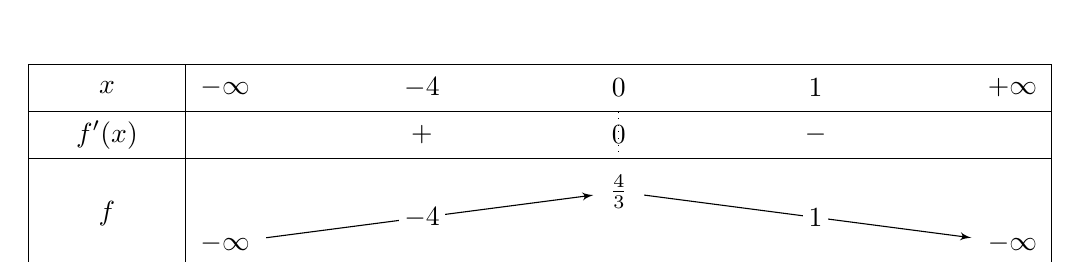
\begin{tikzpicture}
            \tkzTabInit[espcl=5]{$x$/0.6,$f'(x)$/0.6,$f$/1.4}{$-\infty$,$0$,$+\infty$}
            \tkzTabLine{,+,z,-,}
            \tkzTabVar{-/$-\infty$, +/$\frac{4}{3}$, -/$-\infty$}
            \tkzTabVal{1}{2}{0.5}{$-4$}{$-4$}
            \tkzTabVal{2}{3}{0.5}{$1$}{$1$}
        \end{tikzpicture}
    \end{center}
    $\mathbb{R}$ est stable par $f$, $(u_n)$ est bien définie.\\
    Soit $l\in\mathbb{R}$. On a $f(l)=l \iff \frac{1}{3}(4-l^2) = l \iff l^2 + 3l - 4 = 0$. $r_1 = 1$, $r_2 = -4$.\\
    Les points fixes de $f$ sont donc en $-4$ et $1$.\\
    On remarque que $]-\infty, -4]$ est un intervalle stable par $f$ sur lequel $f$ est monotone.\\[0.2cm]
    \underline{Cas n°1 : $u_0 \in \{-4,1\}$}\\
    Remarque : Lorsque $u_0 \in \{1,4\}$, on a $u_1 \in \{-4,1\}$ : même raisonnement.\\
    Ce sont les points fixes de $f$ : $(u_n)$ est convergente vers $u_0$.\\[0.4cm]
    \underline{Cas n°2 : $u_0 \in ]-\infty, -4[$}.\\
    Remarque : Lorsque $u_0\in]4,+\infty[$, on a $u_1\in]-\infty, -4[$ : même raisonnement.\\
    On a $f$ croissante sur $]-\infty,-4]$, alors $(u_n)$ est monotone sur cet intervalle.\\
    De plus, $u_1 - u_0 = \frac{1}{3}(4-u_0^2) - u_0 < 0$, alors $(u_n)$ est décroissante.\\
    Enfin, on a que $u_0$ est inférieur à tout point fixe de $f$ : $u$ ne peut pas converger, elle diverge vers $-\infty$\\[0.4cm]
    \underline{Cas n°3 : $u_0 \in ]-4,4[$}.\\
    On a que $]-4,4[$ est un intervalle stable par $f$ sur lequel $f$ est croissante puis décroissante.\\
    De plus, $\forall x\in]-4,1[, ~ f(x)-x > 0$ et $\forall x \in ]1,4[, ~ f(x)-x < 0$ et pour $x=1, ~ f(x)-x=0$.\\
    Ainsi, $(u_n)$ est croissante sur $]-4,1]$ et décroissante sur $[1,4[$.\\
    Aussi, $\forall n\in\mathbb{N}, u_n \in[2,4[ \Rightarrow u_{n+1} \in ]-4,0]$ et $\forall n \in\mathbb{N}, ~ u_n\in ]1,2] \Rightarrow u_{n+1} \in [0,1[$\\
    Et : $\forall n \in\mathbb{N}, ~ u_n \in [0,1] \Rightarrow u_{n+1} \in [1,\frac{4}{3}]$.\\
    Par théorème de la limite monotone, $(u_n)$ converge vers 1.\\
    \qed
\end{tcolorbox}

\addcontentsline{toc}{section}{Modes de définition particulier d'une suite}
\addcontentsline{toc}{section}{\protect\numberline{}Exercice 13.17}

\section*{Exercice 13.18 [$\blacklozenge\blacklozenge\blacklozenge$]}
\begin{tcolorbox}[enhanced, width=7.6in, center, size=fbox, fontupper=\large, drop shadow southwest]
    Prouver que pour tout $n\in\mathbb{N}^*$, il existe un unique $x_n>0$ tel que $x^n_n + x_n = 3$. Prouver que $(x_n)$ converge et déterminer sa limite.\\
    Soit $n\in\mathbb{N}^*$ et soit $f_n : x\mapsto x^n + x$. $f_n$ est dérivable et $f'_n: x \mapsto nx^{n-1} + 1$ on a :
    \begin{center}
        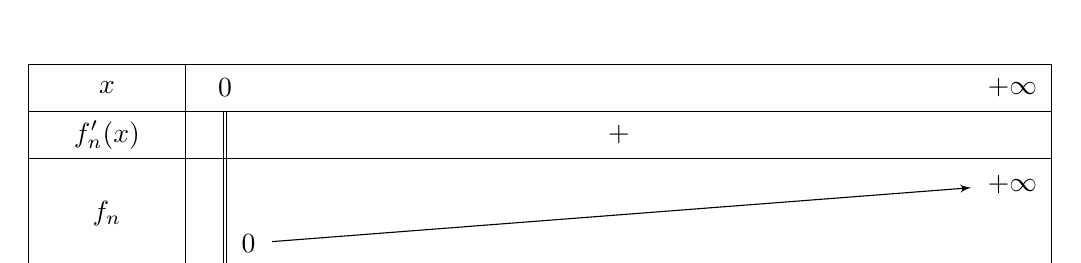
\begin{tikzpicture}
            \tkzTabInit[espcl=10]{$x$/0.6,$f_n'(x)$/0.6,$f_n$/1.4}{0,$+\infty$}
            \tkzTabLine{d,+}
            \tkzTabVar{D-/$0$, +/$+\infty$}
        \end{tikzpicture}
    \end{center}
    On a que $f_n$ est continue et strictement croissante sur $]0, +\infty[$, de plus $f_n$ prend ses valeurs dans $]0, +\infty[$. D'après le TVI, il existe une unique solution à l'équation $x_n^n +x_n = 3$. La suite $(x_n)$ est donc bien définie.\\
    De plus, puisque $f_n(1)=2<f_n(x_n)$, on a que $x_n>1$ pour tout $n\in\mathbb{N}$.\\
    De plus, il est évident que $x_n<3$ pour tout $n\in\mathbb{N}$.\\
    Montrons que $(x_n)$ est décroissante. Soit $n\in\mathbb{N}^*$. On a :
    \begin{equation*}
        3 = x^{n+1}_{n+1}+x_{n+1} = x_{n+1}f_n(x_{n+1}) - x_{n+1}^2 + x_{n+1}
    \end{equation*}
    Ainsi, $f_n(x_{n+1})=\frac{3 +x_{n+1}^2  - x_{n+1}}{x_{n+1}}=x_{n+1} - 1 + \frac{3}{x_{n+1}}<3$ car $x_n\in[1,3]$.\\
    Alors $f_n(x_{n+1})<3=f_n(x_n)$. On a bien montré que $(x_n)$ est décroissante.\\
    La suite $(x_n)$ est décroissante et minorée par 1, d'après le TLM, elle converge vers une limite $l\geq1$.\\
    Supposons que $l>1$.\\
    Alors : $x_n^n = e^{n\ln(x_n)} \to +\infty$ car $x_n \to l$.\\
    Donc $x_n^n + x_n \to +\infty$, ce qui est absurde : $\forall n \in \mathbb{N}^*, ~ x_n^n + x_n = 3 \to 3$.
    Ainsi, $(x_n)$ converge vers 1.\\
    \qed
\end{tcolorbox}
\end{document}
 
